\chapter{循环神经网络加速技术基础}

\section{循环神经网络的典型结构}
循环神经网络是一种专门针对序列数据进行建模的神经网络模型。有别于前馈神经网络,卷积神经网络等“静态模型”,循环神经网络在结构上拥有循环
自连接的反馈机制,这使得模型当前的输出不仅取决于当前输入,还与当前的状态有关。通过对状态的存储与更新,循环神经网络能够有效的建模动态系统。
理论上,任何图灵可计算的函数都可以用有限维的循环网络近似。尽管循环神经网络功能强大,但是高昂的训练成本阻碍了循环神经网络的实际应用。
一方面,固定有序的前向传播过程只能遵循序列顺序先后计算,因此通过时间的反向传播无法并行计算;另一方面,梯度消失和梯度爆炸问题在循环神经网络
的训练过程中尤为突出,这导致其学习长期依赖关系变的困难。随着理论研究的发展和算力的提升,以上问题都得以解决。借助第三次人工智能浪潮
循环神经网络重新焕发出勃勃生机,目前,循环神经网络已经广泛应用于自然语言处理等相关领域。

\subsection{普通循环神经网络}
普通循环神经网络是最简单的循环神经网络结构,主要包括输入层,隐藏层和输出层。输入层对输入进行特征提取并映射为固定长度的向量,隐藏层将输入信息
和前一时刻的状态转化为新的状态,输出层根据网络存储的状态解码并完成输出。其中隐藏层包含记忆信息以及记忆更新的规则,是循环神经网络中最重要的
结构。
常见的循环神经网络结构如图\ref{fig:rnn}所示,权重矩阵\(U, W, V\)分别表示输入到到隐藏,隐藏到隐藏,隐藏到输出之间的连接,向量\(x, h, o\)分别表示输入单元,
隐藏单元和输出单元,这些单元及其相互连接形成网络。相比于其他网络模型的单向信息传递,循环神经网络引入环状结构实现了从输入到输出的双向信息
流动。一些符合训练准则的信息将会通过循环的方式长期保存在网络状态中,并根据输入序列特征进行适时唤醒记忆。当网络记忆的信息足够丰富时,循环神经
网络不仅能准确的预测输出,并且能大致恢复输入序列。自编码器框架就是基于此原理而产生,其能根据记忆的状态信息选择重要的输入并近似复制到输出,
实现特征学习或降维。图中左侧为循环神经网络回路原理图,黑色方块表示回路中单个时间步的延迟,即时刻t-1的状态会影响时刻t的状态。图中右侧为
循环神经网络按时间展开的计算图,展开是指将左侧的回路结构映射为右侧的包含重复组件的结构,展开的深度取决与序列的长度。循环神经网络展开结构图
显式的数据流动路径描述了信息是如何在时间上向前和向后传递的。
\begin{figure}
	\centering
	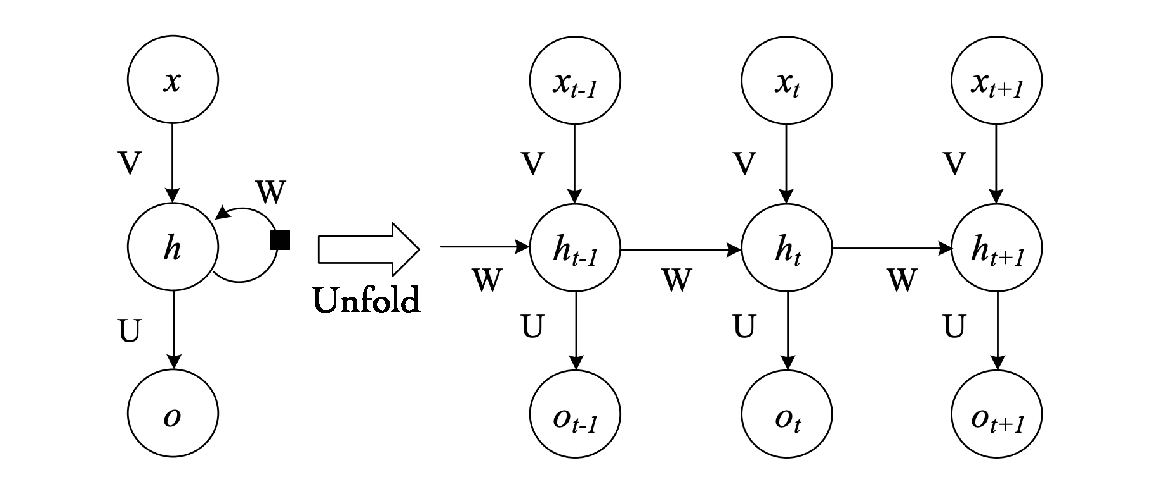
\includegraphics[width=0.8\columnwidth]{RNN_struct.eps}
	\caption{普通循环神经网络结构图}
	\label{fig:rnn}
\end{figure}

循环神经网络的数学模型为式\ref{eq:rnn}, 其中\(g\), \(f\)分别表示隐藏层和输出层的激活函数。在循环神经网络中\(g\)一般选用\(sigmoid\),\(tanh\)
等饱和性激活函数以避免训练过程中可能出现的梯度爆炸问题。函数表达式除了描述模型输入与输出的关系外,还规定了循环神经网络内部结构的
一般特性:

(1)状态的长度固定,即模型的记忆容量有限。\(h_t\)作为过去序列与任务相关方面的有损摘要,只能根据训练准则选择性的保留过去序列的某些方面特质。

(2)模型单个时间步的输入是固定的。无论序列的长度,模型每个时刻始终具有相同大小的输入,状态转移也只能从一种状态转移到下一种状态,
而不是在可变长度的输入序列或历史状态上进行操作。

(3)每个时间步使用相同参数的相同转移函数,即输出的每一项是对先前输出应用相同的更新规则而产生的。更新规则在时间上共享,模型能够表示序列间的相互影响。
相比在所有时间步均建立独立的学习模型,单一的共享模型在非训练集的序列上具有良好的泛化能力。

\begin{equation}\label{eq:rnn}
	\begin{split}
		h_{t} &= g(W h_{t-1} + U x_{t})	\\
		y_{t} &= f(V h_{t})						
	\end{split}
\end{equation}

循环神经网络的训练采用通过时间的反向传播算法(Back-propagation through time,BPTT)。梯度计算首先将一段序列依次送入模型进行前向传播,
保存前向传播过程中的各个状态并计算最终的损失函数;然后,计算梯度并沿时间反向更新权重参数。由于循环网络的计算涉及相同函数的多次组合,
无论沿时间正向或者反向,当需要捕获的依赖关系需要跨越很长的时间尺度时,输入和输出会出现极端的非线性行为。具体的,如果雅可比矩阵的最大特征值
小于1,多次连乘后梯度会趋于0,梯度消失会使得模型参数无法更新,梯度下降算法永远不会收敛到最优解;如果雅可比矩阵的最大特征值大于1,那么随着
时间跨度的增大,梯度也将越来越大,最终会导致权重剧烈改变,学习也变得不稳定。梯度消失和梯度爆炸问题使得循环神经网络学习序列的长期依赖
关系变得困难, 目前,研究人员提出了一些降低学习长期依赖难度的方法,在某些情况下循环神经网络可以学习跨越百步的依赖关系,尽管取得了很大的进步
但是,如何学习更长时间的依赖关系仍然是深度学习领域的一个主要挑战。


\subsection{长短期记忆神经网络}
长短期记忆神经网络(Long short-term memory,LSTM)是目前应用范围最广的一种循环神经网络,相比简单的循环架构,LSTM能更容易的学习到长期依赖。
其结构中存在多层循环,除了外部的循环外,内部还存在“LSTM细胞”自循环。多层循环使得时间路径增加,梯度消失的可能性被大大降低,因此更深的循环神经
网络架构也得以实现\citing{}。

LSTM网络结构如图\ref{fig:lstm}所示,输入信息需要经过多条数据路径并进行复杂的加工处理才能最终到达隐藏层,这些位于数据路径中的“门”控制着信息的通过率。
其值越接近1表示该信息越需要被记忆,越接近0表示信息应该迅速被丢弃。通过控制信息的通过率,网络能够在较长的时间内持续积累线索,并且尽量少的受
干扰信息影响,因此累积的时间尺度可以动态的调节。LSTM网络中的门主要包括输入门\(i\),遗忘门\(f\)和和输出门\(o\),网络的输入信息包括细胞态\(c_{t-1}\),
状态\(h_{t-1}\)以及输入\(x_t\)。

在LSTM网络的前向传播过程中,首先当前的输入\(x_t\)和上一时刻的状态\(h_{t-1}\)会共同生成遗忘门的通过率,上一时刻的细胞态\(c_{t-1}\)会在此门
的控制下选择性的通过。然后,在输入门的控制下,输入信息中的重要线索会被合并到新的细胞状态中。最后细胞当前的状态会通过输出门进行最终的
筛选并产生新的状态。以上输入信息和记忆信息在三个门控单元的层层作用下,序列中符合学习经验的信息将会在很长的时间尺度内被收集起来,实现长期记忆,
而无关的信息所形成的短期记忆则会随着时间流逝迅速被遗忘。图中上半部分LSTM网络的循环图,图中清晰的展示了细胞态和状态的时间回路;图中下半部分为
LSTM网络的展开图,同一组件按时间顺序依次排开形成时间维度的信息流动路径,图中不仅描述了单个时间步信息如何被处理,还描述了相邻时间步之间数据如何
被衔接。

\begin{figure}
	\centering
	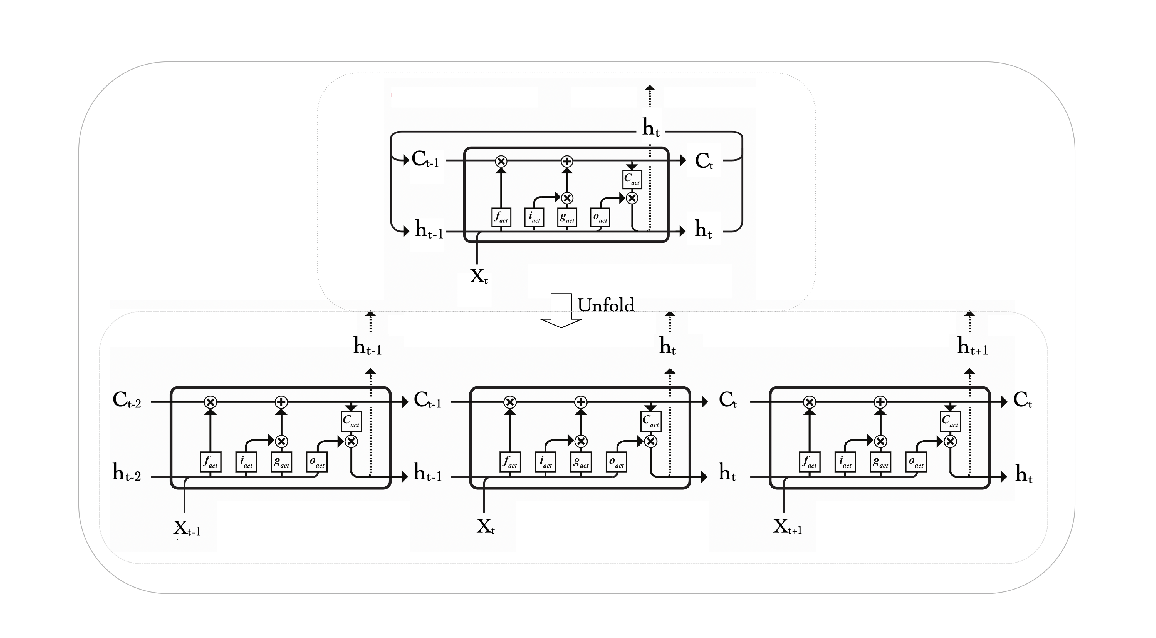
\includegraphics[width=1\columnwidth]{LSTM_struct.eps}
	\caption{LSTM结构图}
	\label{fig:lstm}
\end{figure}

LSTM网络的数学模型为式\ref{eq:lstm},该表达式详细说明了LSTM网络从t=1到t=T的计算流程。其中\(W\)表示权重矩阵,\(b\)表示偏置向量,\(\odot\)运算符
表示向量按位相乘,\(+\)运算符表示向量按位相加,符号\(i\),\(f\),\(o\),\(c\)分别表示输入门,遗忘门,输出门和细胞状态。向量的按位乘法实际上表示
信息在门控单元的筛选下选择性的通过,门控单元的通过率不是固定不变的,而是根据上下文进行动态的调节。向量加法实际上可理解位信息合并的过程,
多条信息通路汇聚后信息通过简单的加和操作完成了信息的整合。

\begin{equation}\label{eq:lstm}
	\begin{split}
		i_t &= \sigma(W_{ix} x_t + W_{ih} h_{t-1} + b_i)	\\
		f_t &= \sigma(W_{fx} x_t + W_{fh} h_{t-1} + b_f)	\\
		g_t &= \tanh(W_{cx} x_t + W_{ch} h_{t-1} + b_c)					\\
		c_t &= f_t \odot c_{t-1} + g_t \odot i_t							\\	
		o_t &= \sigma(W_{ox} x_{t} + W_{oh} h_{t-1} + b_o)	\\
		h_t &= o_t \odot \tanh(c_{t})											\\												
	\end{split}
\end{equation}


\subsection{回声状态网络}
回声状态网络(Echo state network,ESN)是一种基于储层计算(reservoir computing)的神经网络,它通过固定循环矩阵巧妙的避免了循环神经网络
训练过程中梯度消失和梯度爆炸的问题,广泛应用于序列预测和动态系统建模。由于其易于训练,基于回声状态网络搭建的深度循环神经网络能够实现并应用,
这显著的增强循环神经网络学习和预测能力。此外,相比于其他循环神经网络,ESN结构更加简单,物理意义也易于解释。因此本文以回声状态网络为例,
提出并设计针对循环神经网络前向传播过程的加速系统,并将该系统基于FPGA硬件实现。

回声状态网络结构如图\ref{fig:esn}所示,其由输入层\(u\),隐藏层\(x\)(储备层)和输出层\(y\)组成。输入层将输入投影到高维的状态空间,信息的特征被
充分的提取并且变得线性可分。隐藏层由大量的神经元组成,数量通常达到几百或上千,这在其他种类的循环神经网络中几乎不可能实现。数量庞大的神经元
通过“回声”完成对输入序列动态特性的记忆,但是记忆的能力并不是来自于学习训练数据中的经验,而是自然形成。回声状态网络中的输入连接权重\(W_{in}\)
和隐藏层的自循环权重\(W\)在初始化阶段随机生成,在训练过程中始终保持固定不变,因此这两部分连接权重不能通过学习来获得。模型的记忆能力与
求解问题无关,这极大的降低了学习的成本。输出层的连接权重是ESN网络中唯一可以学习的参数,通过选择与任务高度相关的记忆及其变换方式,模型
可以满足特定系统的动力学要求。

\begin{figure}
	\centering
	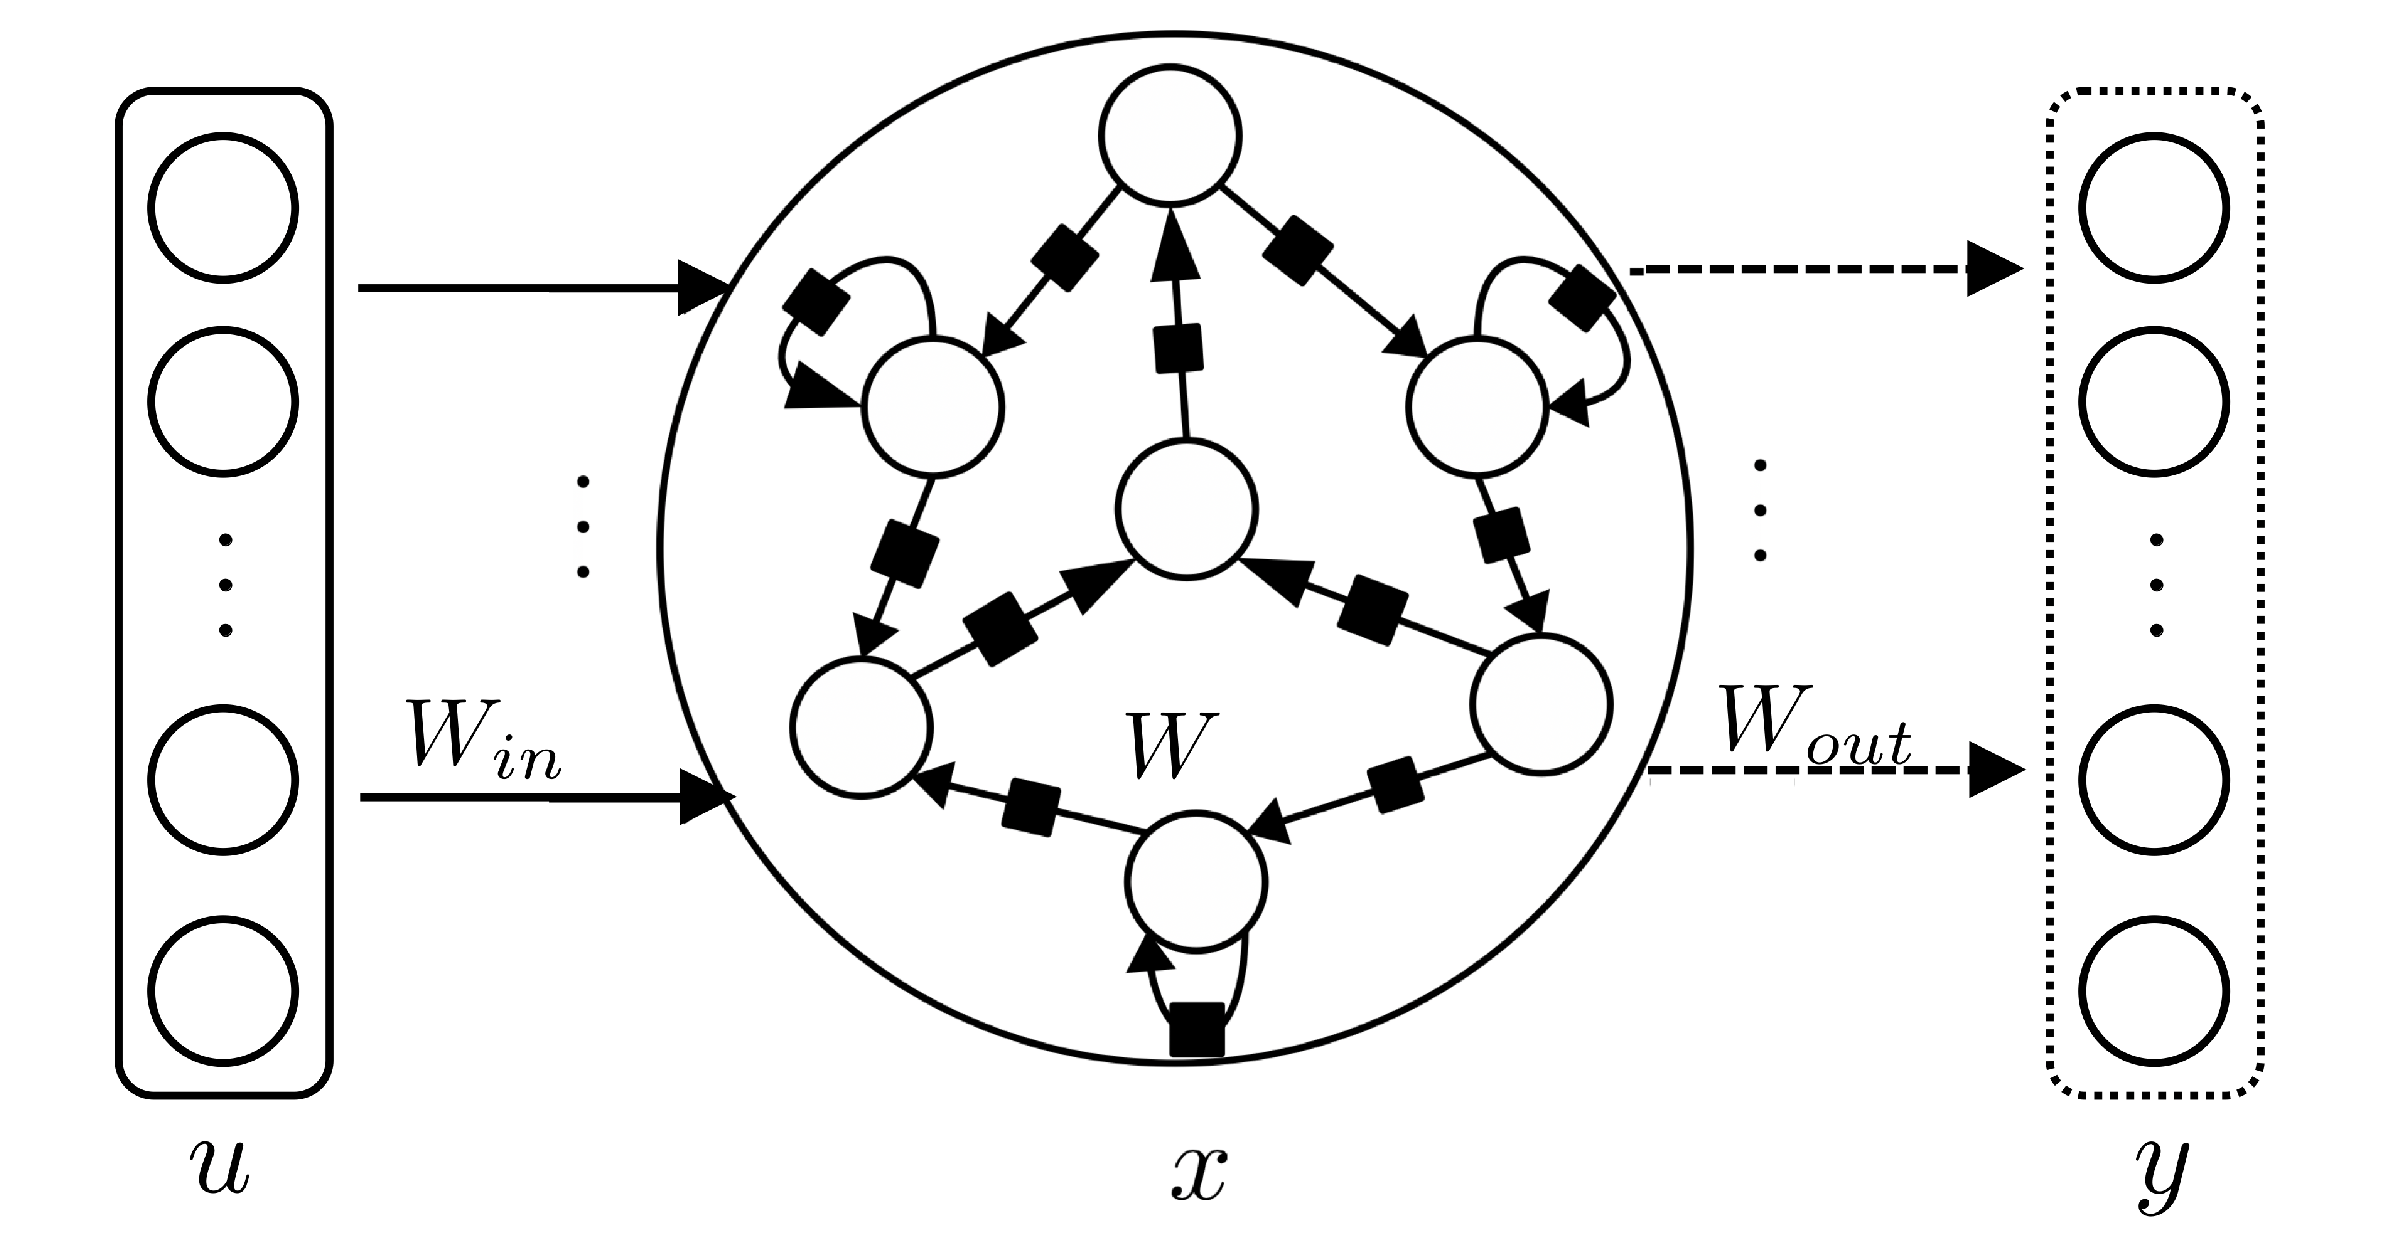
\includegraphics[width=0.7\columnwidth]{ESN_struct.eps}
	\caption{ESN结构图}
	\label{fig:esn}
\end{figure}

回声状态网络的基本数学模型为式\ref{eq:esn},其中\(x\in \mathbb{R}^n\)表示隐藏层神经元数量为n,\(u \in \mathbb{R}^{n_{in}}\)和\(y \in \mathbb{R}^{n_{out}}\)
分别表示模型的单个时间步的输入为\(n_{in}\)维,输出为\(n_{out}\)维;权重矩阵\(W_{in} \in \mathbb{R}^{n \times n_{in}}\),\(W\ \in \mathbb{R}^{n \times n}\)和\(W_{out} \in \mathbb{R}^{n_{out} \times n}\)
分别表示输入层到隐藏层,隐藏层到隐藏层,隐藏层到输出层神经元之间的相互连接。\(W_{in}\)和\(W\)随机生成,不可训练。为解决系统的稳定性问题
需要设定\(W\)的谱半径\(SR < 1\)。为保证网络能够记忆足够的动态特性,隐藏层通常拥有大量神经元来超额记忆任务所需要记住的数据。随机性和冗余性
使得网络的训练成本降低,模型的记忆能力增强,但是随之而来的是在处理实际问题过程中网络前向传播过程中计算量增大,推理延迟变高。计算与性能的
平衡是以回声状态网络为代表的循环神经网络在实际应用过程中面临的一个重要挑战。
\begin{equation}\label{eq:esn}
	\begin{split}
		x_{t} &= f(W x_{t-1} + W_{in} u_{t})	\\
		y_{t} &= W_{out} x_{t}				
	\end{split}
\end{equation}

回声状态网络训练一般采用简单的线性回归方法,通过最小化均方误差来获得输出的连接权值。为解决简单线性回归过程中可能出现的矩阵病态问题,目前广泛采用
岭回归方法,具体的训练方法如式\ref{eq:lrm}。其中\(X\) = \{\(x_1\),\(x_2\),...,\(x_t\)\}是前向传播过程中状态连续采样的集合,\(Y_{target}\)是
是与状态集合一一对应的真实输出值,\(I\)是单位矩阵,\( \lambda > 0\)作为规则化因子可以增加模型的泛化能力。总体上回声状态网络的训练包括状态采样和
线性回归两大过程,相较传统的循环神经网络的BPTT算法,具有收敛速度快,计算复杂度低等特点。
\begin{equation}\label{eq:lrm}
	W_{out} = Y_{target} X^{T}(XX^{T} + \lambda I)^{-1}
\end{equation}

回声状态网络拥有循环神经网络的一般共性及其优势。结构上,隐藏层在时间维度存在自循环结构;功能上,它们能有效的捕获动态系统的时序特性;计算特性上,
前向传播过程中包含大量的矩阵向量乘法,属于计算和存储都密集的应用。在保有优势的同时,回声状态网络也继承了循环状态网络所拥有的普遍劣势。为保证模型
能够记忆足够丰富的动态特性并获得足够精细的预测效果,网络中一般存在大量的隐藏层神经元,相应的表示起连接关系的权重矩阵的规模也将呈平方式增长。参数量和
计算量增长所带来的存储压力和计算延迟会阻碍循环神经网络的实际应用。回声状态网络降低训练成本的代价是拥有规模巨大的神经元数量,这将显著放大劣势。
以上,回声状态网络是具有代表性的一种循环神经网络,研究其前向传播的加速技术对于其他种类的循环神经网络的加速极具参考价值。实际上,本文所采用的针对回声
状态网络的压缩算法普遍适用于其他循环神经网络如LSTM,GRU等,本文所提出的循环神经网络加速系统也具有普遍适用性,但是本文仅以回声状态网络的加速系统为例,因为
其结构简单,训练成本低且拥有广泛的应用前景。
\section{模型压缩与加速算法}
%\subsection{轻量化网络}
神经网络参数和计算量的爆炸式增长会提高模型的预测效果,但是其所带来计算延迟和高功耗问题会严重制约人工智能应用的实际落地。目前神经网络的
前向传播过程存在两种不同层面的加速方法。在算法层面,开发专门针对神经网络的模型压缩算法,主要目的是降低模型的参数量和计算量。在硬件层面,
开发适应神经网络特性的专用加速器,以更好的发挥硬件执行效率和降低运行功耗。实际上,神经网络加速系统的设计往往综合考虑两种方法的优势,以进一步
获取更大的加速效果。本小节简要的介绍几种常用的模型压缩算法,这些算法与本文所采用的压缩算法属于相互独立的工作,但是所采用的基本理论具有相似性。
介绍这些工作旨在说明本文的压缩算法实现成本更小,可以在边缘设备实现,具有明显的优越性。

\subsection{模型稀疏化}

\begin{figure}
	\centering
	\begin{minipage}[t]{0.48\textwidth}
		\centering
		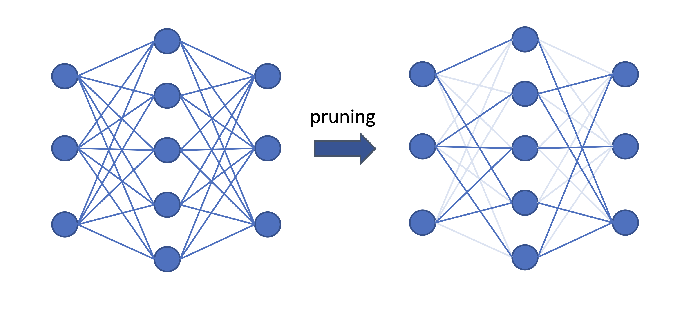
\includegraphics[width=1\columnwidth]{fig_purning.eps}
		\caption{模型剪枝示意图}
		\label{fig:purning}
	\end{minipage}
	\begin{minipage}[t]{0.48\textwidth}
		\centering
		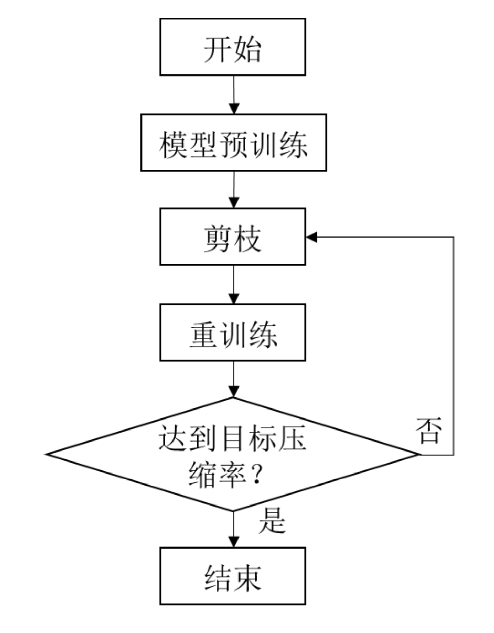
\includegraphics[width=0.6\columnwidth]{fig_purning_alg.eps}
		\caption{剪枝流程图}
		\label{fig:purning_alg}
	\end{minipage}
\end{figure}
模型剪枝是指将网络中一些冗余的神经元删除或将权重矩阵中的一些参数置零,这是目前神经网络模型压缩的常用且有效的方法。模型剪枝的直观效果如图
\ref{fig:purning}所示,剪枝算法会降低神经元之间相互连接的数量,从而精简网络,达到计算加速和压缩存储的目的。模型剪枝一般依据连接或神经元
对模型预测准确率的影响程度,将参数的L-1或L-2范数进行排序,然后将小于设定阈值的参数直接移除。如果选用的剪枝依据不当或者设置的压缩率过高,
模型的预测精度将会受到严重影响,甚至完全无法工作。

模型压缩会不可避免的导致预测精度的下降,剪枝方法在精度损失方面表现的更为突出,尤其是将剪枝方法应用于深度神经网络和循环神经网络时,误差会在空间和
时间维度进行累积。因此剪枝后的模型通常需要再训练,通过微调参数实现对精度的补偿。剪枝算法的具体流程如图\ref{fig:purning_alg}所示。首先,模型会在训练集
上进行预训练,然后依据剪枝阈值对模型初步剪枝并在训练集上完成重训练过程,最后判断剪枝后的模型是否达到目标压缩率,“是”则流程结束,“否”则反复执行
“剪枝-重训练”过程,直到满足压缩率要求。以上“训练-剪枝-再训练”过程通常需要反复迭代,保持压缩模型精度不显著降低的代价是付出了高昂的训练成本。

元素级的细颗粒剪枝使得稠密的权重矩阵变成了具有随机非零值分布的稀疏矩阵,非结构化的稀疏矩阵在进行矩阵乘法时会引入不规则的存储访问和计算模式,
这使得剪枝后的模型无法很好的应用在通用并行处理器中。为解决非结构化稀疏矩阵对硬件不友好的问题,结构化剪枝方法(粗颗粒剪枝)应运而生。
粗颗粒剪枝是指每次剪枝操作将一组权值整体作为剪枝对象,而不是针对每个权值个体。其所带来的益处是非零权值的分布不再具有随机性,而是集中分布在
每一个组里,这有利于解决不规则访存和计算平衡的问题。但是也正由于结构化剪枝严格限制了网络中神经元之间的相互连接,模型的精度会显著下降且难以补偿。
\begin{figure}
	\centering
	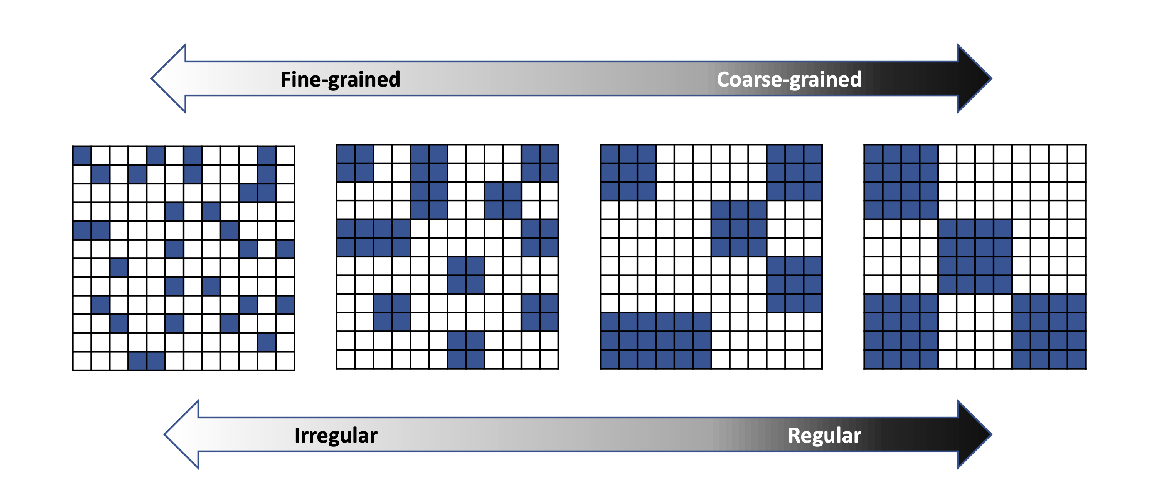
\includegraphics[width=0.8\columnwidth]{fig_purning_structure.eps}
	\caption{剪枝颗粒度与模型结构化程度示意图}
	\label{fig:struc_purn}
\end{figure}

图\ref{fig:struc_purn}展示了剪枝颗粒度和模型结构化程度之间的关系,剪枝颗粒度越小,非零值位置的自由度越高,剪枝后模型的精度也就越高;
剪枝颗粒度越大,非零值的分布就越集中,剪枝后模型在硬件执行时计算效率就越高。找到模型精度和计算效率平衡时剪枝算法面临的一个重要挑战。

%\subsection{数值量化}

\subsection{张量分解}
张量是神经网络的基本组成部分,其处理过程往往需要消耗大量的计算和存储资源,直接对张量进行压缩是一种有效减少网络模型参数量的方法。张量压缩
是指将庞大参数量的张量分解成多个更小的张量,分解后的小张量能够通过一组运算还原为大的张量。张量分解过程是一个信息密集化的过程,其冗余
数据会在分解的过程中被移除或用更简洁的方式被表达。低秩近似是一种常用的二维张量近似方式,其效果如图\ref{fig:lowrank}所示。对于一个秩为
q的方阵\(W \in \mathbb{R}^{n \times n}\),\(W\)可分解维两个矩阵相乘\(W = W_a  W_b\),其中\(W_a\)的大小为\(n \times q\),\(W_b\)的大小为\(q \times n\)。
当\(q << n \)时,权值矩阵的空间复杂度从\(\mathcal{O}(n^2)\)降低到\(\mathcal{O}(2nq)\)。
\begin{figure}
	\centering
	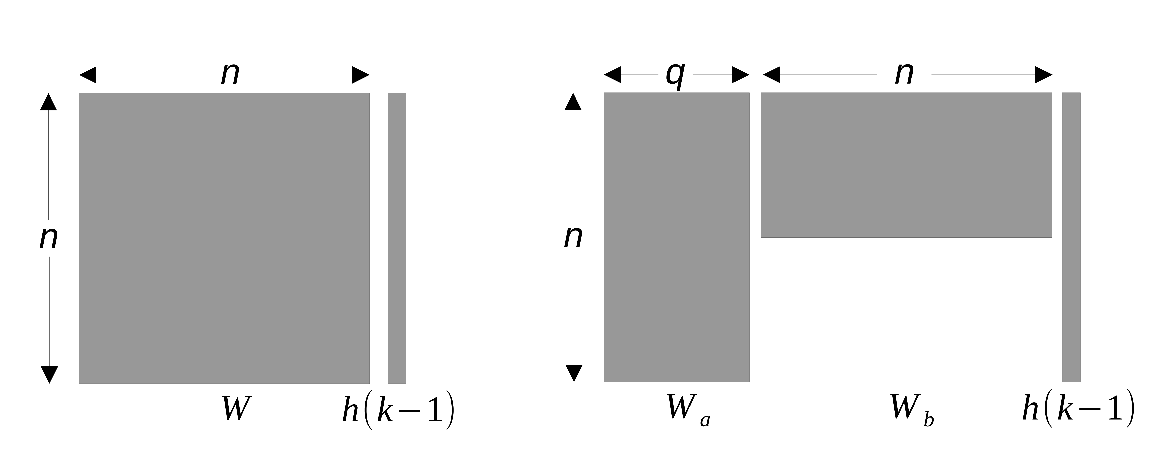
\includegraphics[width=0.8\columnwidth]{low_rank.eps}
	\caption{低秩分解}
	\label{fig:lowrank}
\end{figure}

奇异值分解(singular value decomposition,SVD)经常用于低秩近似和模型降阶中,其可以从包含向量化数据的矩阵中提取最主要的特征。相比于特征值分解只能应用在满秩的
方阵,SVD可以分解任意大小的矩阵,其数学表达为式\ref{eq:SVD},其中\(A \in \mathbb{R}^{m \times n}\)为待分解矩阵,\( U \in \mathbb{R}^{m \times m}\)和\( V \in \mathbb{R}^{n \times n}\)
是酉矩阵,分别由A的左奇异向量和右奇异向量张成。\(\Sigma \in \mathbb{R}^{m \times n}\)是对角矩阵,对角线上的元素是与特征向量相对应的特征值。一般情况下,
特征值(\(\sigma_1, \sigma_2,...,\sigma_k\)),\(k=min(m,n)\)按数值大小排列,数值越大,表示该特征在还原矩阵时影响程度越大。模型降维的过程就是
舍弃不重要的特征向量的过程,剩下的特征向量张成的空间即为降维后的空间。
\begin{equation}\label{eq:SVD}
	A = U  \Sigma   V^T
\end{equation}

本征正交分解(proper othogonal decompositon,POD)是另一种将数据从高维压缩到低维的方法,该方法将相关数据的特征进行分离,在其特征空间构造一组
标准正交基并形成基空间,基空间的维度等于线性无关数据的数量。高维数据可以简单分解为的基向量的线性组合,而线性组合系数的数量往往远小于高维数据的数据个数,
因此,高维数据可以用低维数据进行表示。式\ref{eq:POD}为线性分解的数学表达式,其中\(x_i\)为数据集中的第i个数据,\(\varphi _k\)是基空间中的第k个投影轴(基向量),
\(a(k)\)是线性组合系数。高维数据\(x_i\)本征正交分解后可以用\((a_1,a_2,...,a_r)\)来近似表示。
\begin{equation}\label{eq:POD}
	\begin{split}
		\mathbf{x_i} \approx \sum_{k=1}^{r}a(k) \varphi _k		\\
	\end{split}
\end{equation}
本征空间可以通过奇异值分解(SVD)获得,假设X是由m个数据构成的数据集
\begin{equation}
	X = [x_1,x_2,...,x_m]
\end{equation}
对其进行奇异值分解
\begin{equation}
	X = \Phi   \Sigma  V^T \approx \Phi _r  \Sigma _r  V_r^T
\end{equation}
式中\(\Phi\)是本征空间,\(V\)是投影矩阵,\(\Sigma\)是奇异值矩阵。由于奇异值分解后各个特征向量在原空间的还原过程中贡献程度不同,可以选择前r
个向量作为数据特征空间的基向量。这将大大减小空间的维度,投影坐标的数据个数也将随之减少。高维数据和低维数据的关系如式\ref{eq:proj},其中\(x\)是高维数据,
\(V_r\)是投影矩阵,\(a\)是低维数据。
\begin{equation}\label{eq:proj}
	\mathbf{x} \approx V_r  \mathbf{a}
\end{equation}

\section{硬件加速平台介绍}
在通用计算时代,软件算法和硬件设计是相互分离的,算法直接面向上层应用旨在解决复杂的应用问题和提升应用效果指标,硬件作为算法的最终实现平台,
其设计目的在于高效快速的执行计算和访存操作。不同的设计目的和约束空间导致算法和硬件存在各自的特性,在实际应用过程中往往需要综合考虑软硬件特性和具体场景需求
选择适合算法特性的计算平台或者根据硬件特性进行算法优化。人工智能领域中的神经网络算法不同于传统算法,其模型结构和运算机制不固定,训练和推理过程相互分离,
面对多样化的需求,选择合适的硬件平台显得尤为重要。本文第一章介绍了现有的神经网络硬件计算平台及其优势和劣势,CPU和GPU由于完善的开发环境和实现框架,多用于
神经网络原型设计和模型训练,ASIC适用于成熟算法的大规模应用,FPGA由于其可配置的特点广泛应用在专用架构设计以及神经网络的推理过程。
本文针对边缘应用场景设计实现循环神经网络加速系统,系统受限于资源和功耗约束,需要满足对延迟和模型预测精度的弹性化需求,FPGA恰能满足上述要求。
因此本文以FPGA作为硬件实现平台,设计循环神经网络前向传播算法的专用加速架构并最终实现独立且完整的加速系统。

\subsection{FPGA硬件加速技术}

FPGA是一种半定制化的硬件电路,内部包含可配置逻辑块(configurable Logic Block,CLB),I/O块(I/O Blocks)和互联通路(Routing Channels),
通过更改CLB中的存储的逻辑值和使能不同的片上互联线,FPGA可以快速的实现不同的定制化硬件结构。此外,FPGA还会集成其他常用模块,例如DSP,BRAM,FF等,
丰富的片上资源使得FPGA可以实现更多且更强大的功能。可重构特性和丰富的资源赋予FPGA“算法即芯片”的优势,研究人员可针对算法的特性,设计高效的硬件架构,从电路
层面直接对算法进行优化,充分发挥每一个硬件结构的性能,最终实现特定算法最大程度的加速。同时,FPGA支持大规模的逻辑并行,因此该计算平台特别适合实现
简单且大规模的计算任务,尤其是神经网络算法中的张量计算。并行度的提高使得提升硬件运行频率显得不再迫切,功耗也会因此大大降低,最终相较其他计算平台,
FPGA可以实现更高的能效。

在算法特性已经确定的条件下,实现算法在定制硬件平台上的高效执行需要采用多种技术手段相互协同,FPGA的典型技术包括:

\begin{itemize}
\vspace{4pt}
\item[1.]并行计算:算法程序在通用计算平台上一般串行执行,但是FPGA等计算资源丰富的硬件平台上则可以采用并行计算执行。通过对计算架构进行并行化定制,
不同的计算资源可以同时执行不同的计算部分。并行计算除了要求硬件资源可并行化外,还要求算法存在并行空间,即各并行计算的部分数据不存在时空依赖关系,彼此相互独立。
神经网络中的矩阵-向量乘法中,元素的乘加计算是相互独立的,通过分配多个乘法器和加法器可以实现并行计算。与GPU不同,FPGA中的并行度可以根据算法及应用
需求进行调节,通过对算法进行串行和并行的组合可以更加灵活的处理计算任务。
\vspace{4pt}
\item[2.]定制化存储层级:数据的存储和移动是现代处理器设计中需要重点考虑的因素之一,合适的存储系统不仅能够降低访存延迟,还能减少数据移动,降低
因数据搬运所产生的功耗。由于存储的速度,容量和成本不同,存储系统一般采用多级存储的方式。例如FPGA的存储结构包括片上存储(URAM和BRAM)和片外存储(SDRAM)。
其中片上存储容量小,但由于靠近计算单元,因此数据搬运的成本低,速度快;片外存储容量大,但访存延迟大,数据搬运产生的功耗高。针对计算和存储密集的
人工智能应用,设计高效的存储系统是提高计算性能的必由之路,这需要考虑网络模型的数据特性,合理的划分存储层级以及与计算结构完成高度的协调配合。
面向具体的神经网络模型确定性的存储需求,专用存储架构可以避免复杂的缓存替换策略,各层级的存储结构往往相互独立且容量“精确”。
\vspace{4pt}
\item[3.]流水线技术:流水线技术是FPGA硬件加速中常用的优化方式之一,该技术将一个复杂的运算过程拆分为多个子过程,子过程有序的经过流水线,这样在每个时钟周期都会有数据输出,
达成源源不断的获取输入并处理数据的效果。相较并行计算的空间结构重复,流水线可以实现多个运算的时间重叠,这可以有效提高数据的吞吐率。其所需付出的代价是
在各个子过程间插入寄存器,当流水线划分不合理时,巨额资源的消耗不会换取性能的显著提升。归根结底,流水线技术是一种性能优化技术,它可以在
软件硬件的并行度确定的条件下,再次实现对应用的加速。

\end{itemize}
\subsection{开发工具}
本文采用Xilinx的FPGA板卡及其所提供的开发套件,包括Vivado,Vitis HLS和Vitis嵌入式软件平台。采用基于高级程序语言的HLS(High-Level Synthesis)编程
模型,相较传统的RTL描述如Verilog和VHDL,高层次硬件电路建模能降低开发难度,提升开发效率。经过数十年的发展,HLS已经在相当程度上可以媲美RTL级硬件开发,
尤其是在人工智能领域,由于算法迭代周期短,各种模型结构层出不穷,传统的硬件实现方式已经难以适应敏捷开发的需求。在HLS编程模型下,硬件设计人员可以直接面向
算法开发符合其计算特性的硬件架构,快速创建高性能硬件计算平台;软件开发人员可以专注于高层次的抽象工作,而不必关注底层硬件的实现细节。高层次综合工具
将软件和硬件桥接在一起,大大所短了FPGA的开发周期。
\begin{figure}
	\centering
	\begin{minipage}[t]{0.48\textwidth}
		\centering
		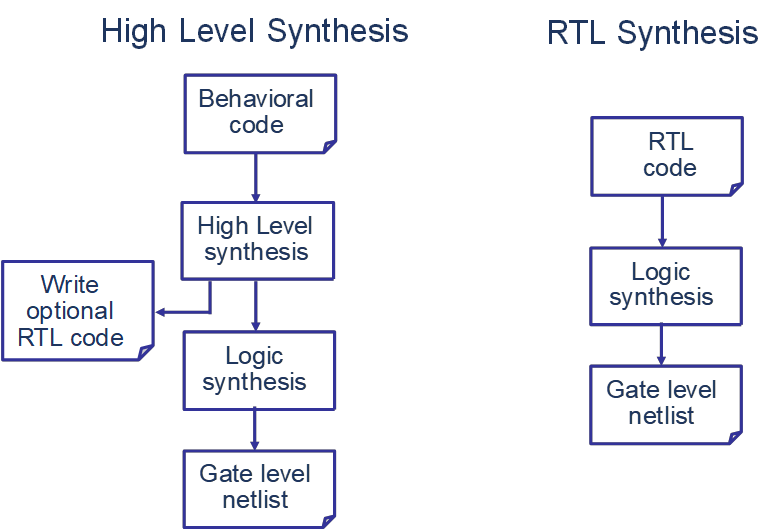
\includegraphics[width=1\columnwidth]{hls.png}
		\caption{HLS流程图}
		\label{fig:hls}
	\end{minipage}
	\begin{minipage}[t]{0.48\textwidth}
		\centering
		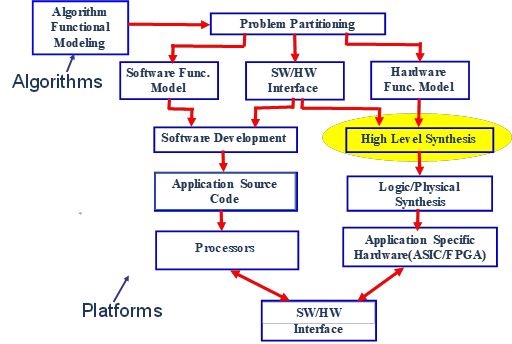
\includegraphics[width=1\columnwidth]{HScodesign.png}
		\caption{基于HLS的软硬件协同示意图}
		\label{fig:hlscodesign}
	\end{minipage}
\end{figure}

HLS的开发流程如图\ref{fig:hls}所示。首先,开发人员需要分析算法的并行度,计算需求以及存储需求等算法特性进行定制化的专用硬件架构设计。需要注意的是,
直接使用软件风格的算法描述作为电路的行为建模尽管能够综合出电路,但通常情况下是低效的。高层次硬件描述应当首先是一种硬件描述,只是抽象层级较高,以至于
和软件描述存在较大的重叠,但是最终的效果却全然不同。描述的对象有输入输出接口,数据位宽,并行化描述,流水线等。在完成硬件架构的行为级建模后,需要进行
行为仿真和综合。行为仿真是指通过对使用高级描述语言所描述的算法功能模块进行编译和验证,找出未覆盖的功能点并据此修正硬件模型。在算法模块功能完整的条件下,
行为综合会将高层次的硬件描述转换为RTL描述,该过程具体可分为调度(scheduling)和绑定(Binding)两大步骤。编译器会根据算法的执行逻辑主动分析数据的并行性及相互
依赖关系,将数据的微操作调度到指定的时间节点,此外,算法的时序控制逻辑也将被提取,如顺序,分支和循环将会以状态机的形式实现。在完成前叙所有流程后,绑定步骤将会
算法的功能模块映射到具体的硬件资源,例如变量,数组,运算,函数将会分别映射为寄存器,BRAM存储器,DSP和协议接口。以上过程即为HLS的原理和实现过程,
在生成RTL描述后,后续的步骤将和传统硬件开发流程相同,此处不再赘述。

\section{本章小结}
本章主要介绍了循环神经网络及其软硬件加速技术基础。首先介绍了几种广泛应用的循环神经网络模型,详细的分析了各个模型的网络结构,推理过程以及其优势劣势,总结出共性和特性,并说明了
循环神经网络在实际应用过程中面临的挑战。接着,本章分别从软件和硬件的角度分别给出解决方案。软件方面主要采用模型压缩技术减轻算法对硬件的计算和存储压力,常用的方法如剪枝和张量分解,
详细的压缩原理和过程被展示出来,其目的一方面在于突显本文所使用的模型压缩算法的优势,另一方面则本对文算法也使用到的相同技术基础做出详细的推导和说明。
在硬件方面,针对本文所使用的硬件实现平台做了详细的介绍,包括FPGA常用的加速技术和高层次硬件描述与综合的原理和过程。
